\documentclass[]{article}
\usepackage{lmodern}
\usepackage{amssymb,amsmath}
\usepackage{ifxetex,ifluatex}
\usepackage{fixltx2e} % provides \textsubscript
\ifnum 0\ifxetex 1\fi\ifluatex 1\fi=0 % if pdftex
  \usepackage[T1]{fontenc}
  \usepackage[utf8]{inputenc}
\else % if luatex or xelatex
  \ifxetex
    \usepackage{mathspec}
  \else
    \usepackage{fontspec}
  \fi
  \defaultfontfeatures{Ligatures=TeX,Scale=MatchLowercase}
\fi
% use upquote if available, for straight quotes in verbatim environments
\IfFileExists{upquote.sty}{\usepackage{upquote}}{}
% use microtype if available
\IfFileExists{microtype.sty}{%
\usepackage{microtype}
\UseMicrotypeSet[protrusion]{basicmath} % disable protrusion for tt fonts
}{}
\usepackage[margin=1in]{geometry}
\usepackage{hyperref}
\hypersetup{unicode=true,
            pdftitle={Home work 1},
            pdfborder={0 0 0},
            breaklinks=true}
\urlstyle{same}  % don't use monospace font for urls
\usepackage{color}
\usepackage{fancyvrb}
\newcommand{\VerbBar}{|}
\newcommand{\VERB}{\Verb[commandchars=\\\{\}]}
\DefineVerbatimEnvironment{Highlighting}{Verbatim}{commandchars=\\\{\}}
% Add ',fontsize=\small' for more characters per line
\usepackage{framed}
\definecolor{shadecolor}{RGB}{248,248,248}
\newenvironment{Shaded}{\begin{snugshade}}{\end{snugshade}}
\newcommand{\KeywordTok}[1]{\textcolor[rgb]{0.13,0.29,0.53}{\textbf{#1}}}
\newcommand{\DataTypeTok}[1]{\textcolor[rgb]{0.13,0.29,0.53}{#1}}
\newcommand{\DecValTok}[1]{\textcolor[rgb]{0.00,0.00,0.81}{#1}}
\newcommand{\BaseNTok}[1]{\textcolor[rgb]{0.00,0.00,0.81}{#1}}
\newcommand{\FloatTok}[1]{\textcolor[rgb]{0.00,0.00,0.81}{#1}}
\newcommand{\ConstantTok}[1]{\textcolor[rgb]{0.00,0.00,0.00}{#1}}
\newcommand{\CharTok}[1]{\textcolor[rgb]{0.31,0.60,0.02}{#1}}
\newcommand{\SpecialCharTok}[1]{\textcolor[rgb]{0.00,0.00,0.00}{#1}}
\newcommand{\StringTok}[1]{\textcolor[rgb]{0.31,0.60,0.02}{#1}}
\newcommand{\VerbatimStringTok}[1]{\textcolor[rgb]{0.31,0.60,0.02}{#1}}
\newcommand{\SpecialStringTok}[1]{\textcolor[rgb]{0.31,0.60,0.02}{#1}}
\newcommand{\ImportTok}[1]{#1}
\newcommand{\CommentTok}[1]{\textcolor[rgb]{0.56,0.35,0.01}{\textit{#1}}}
\newcommand{\DocumentationTok}[1]{\textcolor[rgb]{0.56,0.35,0.01}{\textbf{\textit{#1}}}}
\newcommand{\AnnotationTok}[1]{\textcolor[rgb]{0.56,0.35,0.01}{\textbf{\textit{#1}}}}
\newcommand{\CommentVarTok}[1]{\textcolor[rgb]{0.56,0.35,0.01}{\textbf{\textit{#1}}}}
\newcommand{\OtherTok}[1]{\textcolor[rgb]{0.56,0.35,0.01}{#1}}
\newcommand{\FunctionTok}[1]{\textcolor[rgb]{0.00,0.00,0.00}{#1}}
\newcommand{\VariableTok}[1]{\textcolor[rgb]{0.00,0.00,0.00}{#1}}
\newcommand{\ControlFlowTok}[1]{\textcolor[rgb]{0.13,0.29,0.53}{\textbf{#1}}}
\newcommand{\OperatorTok}[1]{\textcolor[rgb]{0.81,0.36,0.00}{\textbf{#1}}}
\newcommand{\BuiltInTok}[1]{#1}
\newcommand{\ExtensionTok}[1]{#1}
\newcommand{\PreprocessorTok}[1]{\textcolor[rgb]{0.56,0.35,0.01}{\textit{#1}}}
\newcommand{\AttributeTok}[1]{\textcolor[rgb]{0.77,0.63,0.00}{#1}}
\newcommand{\RegionMarkerTok}[1]{#1}
\newcommand{\InformationTok}[1]{\textcolor[rgb]{0.56,0.35,0.01}{\textbf{\textit{#1}}}}
\newcommand{\WarningTok}[1]{\textcolor[rgb]{0.56,0.35,0.01}{\textbf{\textit{#1}}}}
\newcommand{\AlertTok}[1]{\textcolor[rgb]{0.94,0.16,0.16}{#1}}
\newcommand{\ErrorTok}[1]{\textcolor[rgb]{0.64,0.00,0.00}{\textbf{#1}}}
\newcommand{\NormalTok}[1]{#1}
\usepackage{graphicx,grffile}
\makeatletter
\def\maxwidth{\ifdim\Gin@nat@width>\linewidth\linewidth\else\Gin@nat@width\fi}
\def\maxheight{\ifdim\Gin@nat@height>\textheight\textheight\else\Gin@nat@height\fi}
\makeatother
% Scale images if necessary, so that they will not overflow the page
% margins by default, and it is still possible to overwrite the defaults
% using explicit options in \includegraphics[width, height, ...]{}
\setkeys{Gin}{width=\maxwidth,height=\maxheight,keepaspectratio}
\IfFileExists{parskip.sty}{%
\usepackage{parskip}
}{% else
\setlength{\parindent}{0pt}
\setlength{\parskip}{6pt plus 2pt minus 1pt}
}
\setlength{\emergencystretch}{3em}  % prevent overfull lines
\providecommand{\tightlist}{%
  \setlength{\itemsep}{0pt}\setlength{\parskip}{0pt}}
\setcounter{secnumdepth}{0}
% Redefines (sub)paragraphs to behave more like sections
\ifx\paragraph\undefined\else
\let\oldparagraph\paragraph
\renewcommand{\paragraph}[1]{\oldparagraph{#1}\mbox{}}
\fi
\ifx\subparagraph\undefined\else
\let\oldsubparagraph\subparagraph
\renewcommand{\subparagraph}[1]{\oldsubparagraph{#1}\mbox{}}
\fi

%%% Use protect on footnotes to avoid problems with footnotes in titles
\let\rmarkdownfootnote\footnote%
\def\footnote{\protect\rmarkdownfootnote}

%%% Change title format to be more compact
\usepackage{titling}

% Create subtitle command for use in maketitle
\newcommand{\subtitle}[1]{
  \posttitle{
    \begin{center}\large#1\end{center}
    }
}

\setlength{\droptitle}{-2em}
  \title{Home work 1}
  \pretitle{\vspace{\droptitle}\centering\huge}
  \posttitle{\par}
  \author{}
  \preauthor{}\postauthor{}
  \date{}
  \predate{}\postdate{}


\begin{document}
\maketitle

\subsection{Homework 1 - to be done as
groups}\label{homework-1---to-be-done-as-groups}

Names: Jonas B H Andersen

Group: Group 3

For deadlines etc, see absalon.

You have to supply botbh the answer (whatever it is: numbers, a table,
plots or combinations thereof), as well as the R or Linux code you used
to make the plots. This should be done using this R markdown template:
we want both the R markdown file and a resulting PDF. For PDF output,
you may have to install some extra programs - R studio will tell you.

Note that:

\begin{enumerate}
\def\labelenumi{\arabic{enumi}.}
\item
  If the R code gives different results than your results, you will get
  severe point reductions or even 0 points for the exercise
\item
  Some questions may request you to use R options we have not covered
  explicitly in the course: this is part of the challenge
\item
  While this is a group work, we expect that everyone in the group will
  have understood the group solution: similar or harder question might
  show up in the individual homework. So, if something is hard, it means
  you need to spend more time on it
\item
  The results should be presented on a level of detail that someone else
  could replicate the analysis.
\end{enumerate}

For statistical tests, you have to:

\begin{enumerate}
\def\labelenumi{\arabic{enumi})}
\item
  Motivate the choice of test
\item
  State exactly what the null hypothesis is (depends on test!)
\item
  Comment the outcome: do you reject the null hypothesis or not, and
  what does this mean for the actual question we wanted to answer
  (interpretation)?
\end{enumerate}

\subsubsection{Question 1}\label{question-1}

Install the package babynames and look at the data babynames:

\begin{Shaded}
\begin{Highlighting}[]
\KeywordTok{install.packages}\NormalTok{(}\StringTok{"babynames"}\NormalTok{)}
\end{Highlighting}
\end{Shaded}

\begin{Shaded}
\begin{Highlighting}[]
\KeywordTok{library}\NormalTok{(babynames)}
\KeywordTok{head}\NormalTok{(babynames)}
\end{Highlighting}
\end{Shaded}

\begin{verbatim}
## # A tibble: 6 x 5
##    year sex   name          n   prop
##   <dbl> <chr> <chr>     <int>  <dbl>
## 1 1880. F     Mary       7065 0.0724
## 2 1880. F     Anna       2604 0.0267
## 3 1880. F     Emma       2003 0.0205
## 4 1880. F     Elizabeth  1939 0.0199
## 5 1880. F     Minnie     1746 0.0179
## 6 1880. F     Margaret   1578 0.0162
\end{verbatim}

\begin{enumerate}
\def\labelenumi{\alph{enumi})}
\item
  List the top 5 female baby names starting with P, regardless of year,
  as a table.
\item
  Using the results from a, plot their occurrences as a function of year
  using a line plot. Comment on your results. If you get strange
  results, explain them and/or improve the plot.
\end{enumerate}

\subsection{Question 2}\label{question-2}

In the same dataset, is the name Arwen significantly more (or less)
common in 2004 vs 1990? Is the change significant? What is the likely
cause? Do not use hard-coding.

\subsection{Question 3}\label{question-3}

Produce the following plot starting from the flowers dataset. A
potentially useful function that you may not have seen: bind\_rows():
merges two tibbles by rows so that the joint tibble becomes longer, not
wider 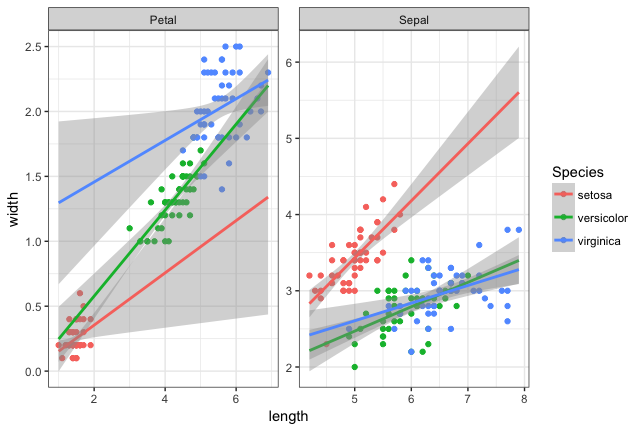
\includegraphics{example.png}

\subsection{Question 4}\label{question-4}

We are given a file with binding sites of a certain transcription
factor, made with the ChIP-seq technique (you will hear a lot more about
the technique later in the course) by a collaborator. In the homework
directory, there is a data file `chip\_mm5.txt' from the collaborator,
representing binding sites from a Chip-chip experiment, with a column
for chromosome, start, end, and score, where score is how `good' the
binding is. Our collaborator has two hypotheses:

1: Binding scores are dependent on chromosome

2: Binding site widths (end-start) are dependent on chromosome

Can you prove/disprove these two hypotheses statistically?

We first collect data from the Chip-chip experiment

\begin{Shaded}
\begin{Highlighting}[]
\NormalTok{chip<-}\KeywordTok{read_tsv}\NormalTok{(}\StringTok{"data/chip_mm5.txt"}\NormalTok{) }\CommentTok{#read data}
\end{Highlighting}
\end{Shaded}

\begin{verbatim}
## Parsed with column specification:
## cols(
##   chr = col_character(),
##   start = col_integer(),
##   end = col_integer(),
##   score = col_double()
## )
\end{verbatim}

\begin{Shaded}
\begin{Highlighting}[]
\KeywordTok{head}\NormalTok{(chip) }\CommentTok{#show data}
\end{Highlighting}
\end{Shaded}

\begin{verbatim}
## # A tibble: 6 x 4
##   chr     start     end score
##   <chr>   <int>   <int> <dbl>
## 1 chr1  4437288 4437576  606.
## 2 chr1  4437624 4437845  506.
## 3 chr1  4682247 4682767  616.
## 4 chr1  4779329 4779612  469.
## 5 chr1  6227828 6228473  512.
## 6 chr1  9699267 9699761   NA
\end{verbatim}

In order to assertain which test to utilize, we plot the score in a
historgram to see whether we can observe a normal distibution of the
data.

\begin{Shaded}
\begin{Highlighting}[]
\KeywordTok{ggplot}\NormalTok{(chip) }\OperatorTok{+}\StringTok{ }\KeywordTok{geom_histogram}\NormalTok{(}\KeywordTok{aes}\NormalTok{(}\DataTypeTok{x=}\NormalTok{score)) }\OperatorTok{+}\StringTok{ }\KeywordTok{facet_wrap}\NormalTok{(}\OperatorTok{~}\NormalTok{chr) }\CommentTok{# plot distribution of scores across each chromosome}
\end{Highlighting}
\end{Shaded}

\begin{verbatim}
## `stat_bin()` using `bins = 30`. Pick better value with `binwidth`.
\end{verbatim}

\begin{verbatim}
## Warning: Removed 5 rows containing non-finite values (stat_bin).
\end{verbatim}

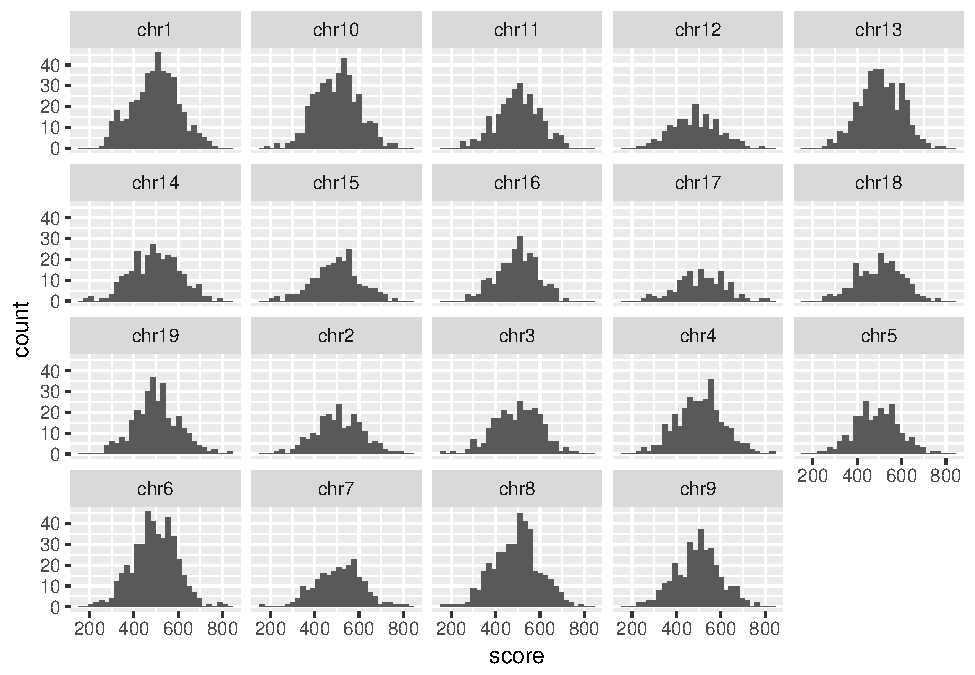
\includegraphics{Hw1_without_solutions_files/figure-latex/unnamed-chunk-3-1.pdf}

We observe a normal distribution of score in each chromosome. In order
to test whether there is a significant difference in binding score in
the chromosomes, we utilize an one-way ANOVA test. H0: there is no
significant difference in means of binding score for each chromosome.
H1: there is a significant difference in means of binding score for each
chromosome.

\begin{Shaded}
\begin{Highlighting}[]
\KeywordTok{oneway.test}\NormalTok{(score }\OperatorTok{~}\StringTok{ }\KeywordTok{as.factor}\NormalTok{(chr), }\DataTypeTok{data=}\NormalTok{chip) }\CommentTok{#Anova test for significance difference between score values across chromosomes}
\end{Highlighting}
\end{Shaded}

\begin{verbatim}
## 
##  One-way analysis of means (not assuming equal variances)
## 
## data:  score and as.factor(chr)
## F = 1.0228, num df = 18.0, denom df = 1797.5, p-value = 0.4298
\end{verbatim}

We cannot reject our null hypothesis since the calculated p-value
\textgreater{} 0.05, therefore we do not observe that there is a
difference in mean binding score across chromosomes.

To test the other hypothesis, we need to modify our data set to include
binding site width.

\begin{Shaded}
\begin{Highlighting}[]
\NormalTok{new_chip<-}\KeywordTok{mutate}\NormalTok{(chip, }\DataTypeTok{site.width =}\NormalTok{ end }\OperatorTok{-}\StringTok{ }\NormalTok{start) }\CommentTok{#create site.width (end - start)}
\KeywordTok{head}\NormalTok{(new_chip) }\CommentTok{#new data}
\end{Highlighting}
\end{Shaded}

\begin{verbatim}
## # A tibble: 6 x 5
##   chr     start     end score site.width
##   <chr>   <int>   <int> <dbl>      <int>
## 1 chr1  4437288 4437576  606.        288
## 2 chr1  4437624 4437845  506.        221
## 3 chr1  4682247 4682767  616.        520
## 4 chr1  4779329 4779612  469.        283
## 5 chr1  6227828 6228473  512.        645
## 6 chr1  9699267 9699761   NA         494
\end{verbatim}

We plot the binding site width in a histogram to ascertain whether the
data is normally distributed

\begin{Shaded}
\begin{Highlighting}[]
\KeywordTok{ggplot}\NormalTok{(new_chip) }\OperatorTok{+}\StringTok{ }\KeywordTok{geom_histogram}\NormalTok{(}\KeywordTok{aes}\NormalTok{(}\DataTypeTok{x=}\NormalTok{site.width)) }\OperatorTok{+}\StringTok{ }\KeywordTok{facet_wrap}\NormalTok{(}\OperatorTok{~}\NormalTok{chr) }\CommentTok{# plot distribution of site width across each chromosome. Not a normal distribution}
\end{Highlighting}
\end{Shaded}

\begin{verbatim}
## `stat_bin()` using `bins = 30`. Pick better value with `binwidth`.
\end{verbatim}

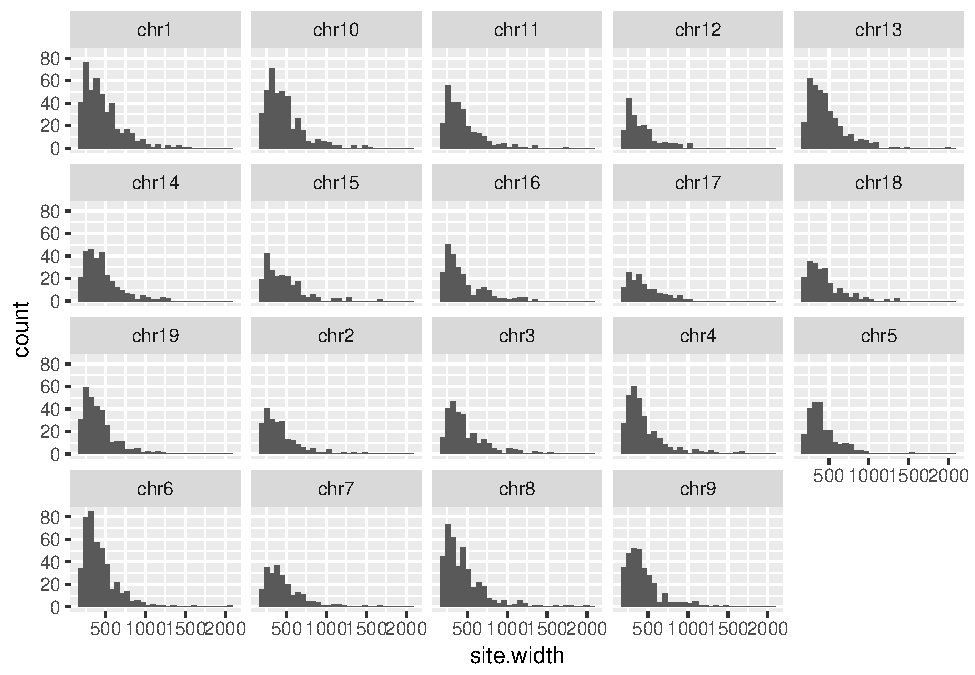
\includegraphics{Hw1_without_solutions_files/figure-latex/unnamed-chunk-6-1.pdf}

The binding site width is not normal distributed in the chromosomes. We
utilize a Kruskal-Wallis test to test our null hypothesis. H0: there is
no significant difference in the mean binding site width for each
chromosome. H1: there is a significant difference in the mean binding
site width for each chromosome.

\begin{Shaded}
\begin{Highlighting}[]
\KeywordTok{kruskal.test}\NormalTok{(site.width }\OperatorTok{~}\StringTok{ }\KeywordTok{as.factor}\NormalTok{(chr), }\DataTypeTok{data=}\NormalTok{new_chip) }\CommentTok{#Kruskal test for significance difference between site width across chromosomes}
\end{Highlighting}
\end{Shaded}

\begin{verbatim}
## 
##  Kruskal-Wallis rank sum test
## 
## data:  site.width by as.factor(chr)
## Kruskal-Wallis chi-squared = 38.536, df = 18, p-value = 0.003288
\end{verbatim}

Calculated p-value \textless{} 0.05 therefore we can reject our null
hypothesis. The alternative hypothesis is proven and there is a
significant difference in binding site width across the chromosomes.


\end{document}
